%%%%%%%%%%%%%%%%%%%%%%%%%%
\subsection{\rev{Rare Disease Extraction}} \label{sec: Results RD Mention Refinement}

\begin{table}[h]
  \centering
  \small
  \setlength{\tabcolsep}{5pt}
  \renewcommand{\arraystretch}{1.18}
  \label{tab:main_results}
  \resizebox{\textwidth}{!}{%
  \begin{tabular}{lcccccccccccc}
    \toprule
    & \multicolumn{4}{c}{\textbf{RareDis}} & \multicolumn{4}{c}{\textbf{MIMIC3-RD Entity}} & \multicolumn{4}{c}{\textbf{MIMIC3-RD Code}} \\
    \cmidrule(lr){2-5}\cmidrule(lr){6-9}\cmidrule(lr){10-13}
    \textbf{Method} & \textbf{P} & \textbf{R} & \textbf{F1} & \textbf{FT} & \textbf{P} & \textbf{R} & \textbf{F1} & \textbf{FT} & \textbf{P} & \textbf{R} & \textbf{F1} & \textbf{FT} \\
    \midrule
    \multicolumn{13}{l}{\textit{Non-LLM Baselines}} \\[1pt]
    Dictionary & \cellcolor[rgb]{1.000,0.679,0.328}0.850 & \cellcolor[rgb]{1.000,0.894,0.740}0.410 & \cellcolor[rgb]{1.000,0.830,0.600}0.550 & {\color{green}\xmark} & \cellcolor[rgb]{1.000,0.900,0.750}0.400 & \cellcolor[rgb]{1.000,0.882,0.716}0.468 & \cellcolor[rgb]{1.000,0.891,0.733}0.431 & {\color{green}\xmark} & \cellcolor[rgb]{1.000,0.936,0.836}0.300 & \cellcolor[rgb]{1.000,0.875,0.700}0.450 & \cellcolor[rgb]{1.000,0.916,0.790}0.360 & {\color{green}\xmark} \\
    BioBERT$^\dagger$ & \cellcolor[rgb]{1.000,0.735,0.418}0.745 & \cellcolor[rgb]{1.000,0.761,0.460}0.695 & \cellcolor[rgb]{1.000,0.749,0.440}0.719 & {\color{red}\cmark} & \cellcolor[rgb]{1.000,0.996,0.990}0.018 & \cellcolor[rgb]{1.000,0.826,0.591}0.559 & \cellcolor[rgb]{1.000,0.993,0.982}0.033 & {\color{red}\cmark} & \multicolumn{3}{c}{\cellcolor[rgb]{0.918,0.910,0.898}\textit{not applicable}} & {\color{red}\cmark} \\
    BioClinicalBERT$^\dagger$ & \cellcolor[rgb]{1.000,0.764,0.464}0.690 & \cellcolor[rgb]{1.000,0.671,0.314}0.867 & \cellcolor[rgb]{1.000,0.723,0.398}0.768 & {\color{red}\cmark} & \cellcolor[rgb]{1.000,0.997,0.992}0.015 & \cellcolor[rgb]{1.000,0.865,0.677}0.473 & \cellcolor[rgb]{1.000,0.994,0.985}0.027 & {\color{red}\cmark} & \multicolumn{3}{c}{\cellcolor[rgb]{0.918,0.910,0.898}\textit{not applicable}} & {\color{red}\cmark} \\
    \midrule
    \multicolumn{13}{l}{\textit{LLM-based (Mistral 24B)}} \\[1pt]
    Zero-Shot & \cellcolor[rgb]{1.000,0.653,0.285}\textbf{0.900} & \cellcolor[rgb]{1.000,0.821,0.580}0.570 & \cellcolor[rgb]{1.000,0.759,0.456}0.700 & {\color{green}\xmark} & \cellcolor[rgb]{1.000,0.970,0.923}0.141 & \cellcolor[rgb]{1.000,0.806,0.548}0.602 & \cellcolor[rgb]{1.000,0.952,0.876}0.228 & {\color{green}\xmark} & \cellcolor[rgb]{1.000,1.000,0.999}0.001 & \cellcolor[rgb]{1.000,0.999,0.996}0.007 & \cellcolor[rgb]{1.000,1.000,0.999}0.002 & {\color{green}\xmark} \\
    RD-RAG & \cellcolor[rgb]{1.000,0.972,0.929}0.130 & \cellcolor[rgb]{1.000,0.658,0.294}\textbf{0.890} & \cellcolor[rgb]{1.000,0.951,0.875}0.230 & {\color{green}\xmark} & \cellcolor[rgb]{1.000,0.990,0.975}0.045 & \cellcolor[rgb]{1.000,0.750,0.442}\textbf{0.716} & \cellcolor[rgb]{1.000,0.982,0.954}0.085 & {\color{green}\xmark} & \cellcolor[rgb]{1.000,0.996,0.991}0.017 & \cellcolor[rgb]{1.000,0.821,0.580}0.570 & \cellcolor[rgb]{1.000,0.994,0.984}0.030 & {\color{green}\xmark} \\
    \textbf{RDMA (ours)} & \cellcolor[rgb]{1.000,0.669,0.311}0.870 & \cellcolor[rgb]{1.000,0.727,0.405}0.760 & \cellcolor[rgb]{1.000,0.701,0.362}\textbf{0.810} & {\color{green}\xmark} & \cellcolor[rgb]{1.000,0.846,0.634}\textbf{0.516} & \cellcolor[rgb]{1.000,0.761,0.460}0.695 & \cellcolor[rgb]{1.000,0.811,0.558}\textbf{0.592} & {\color{green}\xmark} & \cellcolor[rgb]{1.000,0.871,0.690}\textbf{0.460} & \cellcolor[rgb]{1.000,0.798,0.530}\textbf{0.620} & \cellcolor[rgb]{1.000,0.839,0.620}\textbf{0.530} & {\color{green}\xmark} \\
    \bottomrule
  \end{tabular}%
  }
  \caption{\rev{\textbf{LLM-based mining generalizes better across distributions.} We evaluate rare disease extraction across three benchmarks, reporting (P)recision, (R)ecall, F1, and whether fine-tuning (FT) is required. BioBERT and BioClinicalBERT$^\dagger$ are fine-tuned on RareDis~\cite{martinez2022raredis} and evaluated zero-shot on MIMIC-III, testing cross-corpus generalization. \textbf{MIMIC3-RD Entity} measures accurate extraction of rare disease mention spans, while \textbf{MIMIC3-RD Code} measures correct identification of the associated Orphanet code.}}
\end{table}





A major goal of RDMA is to automatically mine rare disease mentions from clinical notes. To the best of our knowledge, the only publicly available benchmark that \rev{contains clinical notes} for this task uses the noisy annotations provided by \cite{dong2023ontology_poor_annotations}. Nonetheless, Given the poor quality of existing annotations, we need to not only effectively mine rare disease mentions, but also provide a framework for efficiently correcting these problematic labels to establish reliable evaluation standards.

\textbf{Baselines.} We evaluate RDMA against \rev{5} baseline approaches: (1) a zero-shot Llama 3.3 70B model \cite{grattafiori2024llama3herdmodels}, (2) a retrieve-and-match dictionary approach using exact string matching, and (3) RAG-RD, a retrieval-augmented generation method specifically designed for rare disease mining, analogous to RAG-HPO \cite{garcia2024_HPORAG}.

\textbf{Evaluation Sets.} To address the annotation quality issues, we created three evaluation sets using 116 clinical notes from MIMIC3 (Table \ref{tab:human_v_rdma&human_stats}): the original processed annotations by \cite{dong2023ontology_poor_annotations}, our human expert corrected labels, and our combined RDMA-human corrected labels. This multi-set evaluation allows us to assess both mining performance and annotation correction capabilities in Step 4 of RDMA (Fig. \ref{fig:RDMAvRAG}).

\textbf{Verification drives rare disease mining performance improvements.} Table \ref{tab:label_correction} demonstrates RDMA's substantially higher precision compared to baseline approaches. The key distinction between RAG-RD and RDMA lies in the tool-based verification step, highlighting LLMs' limitations in directly identifying rare diseases. While we observe that the verification process is imperfect, this finding aligns with recent research \cite{wu2024hybrid} that verification is required for substantially less noisy mining of rare diseases. Given the complexity of clinical notes (with average word lengths in the thousands, as shown in Table \ref{tab:human_v_rdma&human_stats}), RDMA's performance improvements are particularly significant.

\textbf{Accelerating annotation workflows.} RDMA's pipeline supports clinical experts by presenting retrieved candidate entities, contextual information, and previously annotated Orphacodes in a streamlined format. By efficiently identifying entities that require expert review, RDMA addresses the time constraints faced by busy clinicians.
The system employs a two-stage verification process to prioritize cases for human review. First, RDMA compares its mining results with previous annotation attempts, computing pseudo false negatives, false positives, and true positives. Second, a verifier module flags the most disagreeable cases: false negatives that are not rare diseases, false positives that are rare diseases, and true positives that are not rare diseases. This approach focuses expert attention on the most contentious annotations where human judgment is most valuable.
This targeted review process reduces the annotation burden by 63\%, decreasing the number of cases requiring re-review from 333 to 122 (Table \ref{tab:human_v_rdma&human_stats}) while maintaining high agreement with human annotators (Table \ref{tab:rdma_agreement}). For example, in Fig. \ref{fig:ex_annotation}, RDMA identified that "NPH" was incorrectly annotated as a rare disease, revealing its actual context related to insulin resistance—a correction confirmed by human experts. For details on annotation guidelines, please see Appendix \ref{appendix:annotator guidelines}.

\textbf{RDMA identifies overlooked disease mentions.} Table \ref{tab:human_v_rdma&human_stats} shows that RDMA-assisted annotation increases the number of unique rare diseases identified, indicating that at least 10 rare diseases present in the clinical notes were missed during initial human annotation. This demonstrates RDMA's dual functionality as a validation tool that reviews existing annotations and as a discovery mechanism that captures entities overlooked in preliminary mining efforts. We show several qualitative examples of overlooked mentions in Fig. \ref{fig:Top_Corrections} in Appendix \ref{appendix: dataset refinement}.

\textbf{Clear Challenges in Mining Rare Diseases.} We observe several challenges when leveraging RDMA, as illustrated in Fig. \ref{fig:annotator_agreement_qualitative}. First, RDMA can be overly strict in rare disease classification, incorrectly rejecting valid rare diseases when they lack exact matches in the Orphanet database. For example, despite having multiple relevant candidates for "portal vein thrombosis" in Orphanet, RDMA may fail to recognize it as a rare disease due to slight terminology differences. Second, RDMA struggles with negation detection, failing to properly interpret phrases like "which was negative" that negate the presence of a condition, despite being explicitly asked in the prompt to consider negations (Fig. \ref{fig:EntityExtractionPrompt}). These challenges stem from limitations in LLMs' ability to perform nuanced reasoning over clinical text.

\begin{figure}[h]
    \centering
    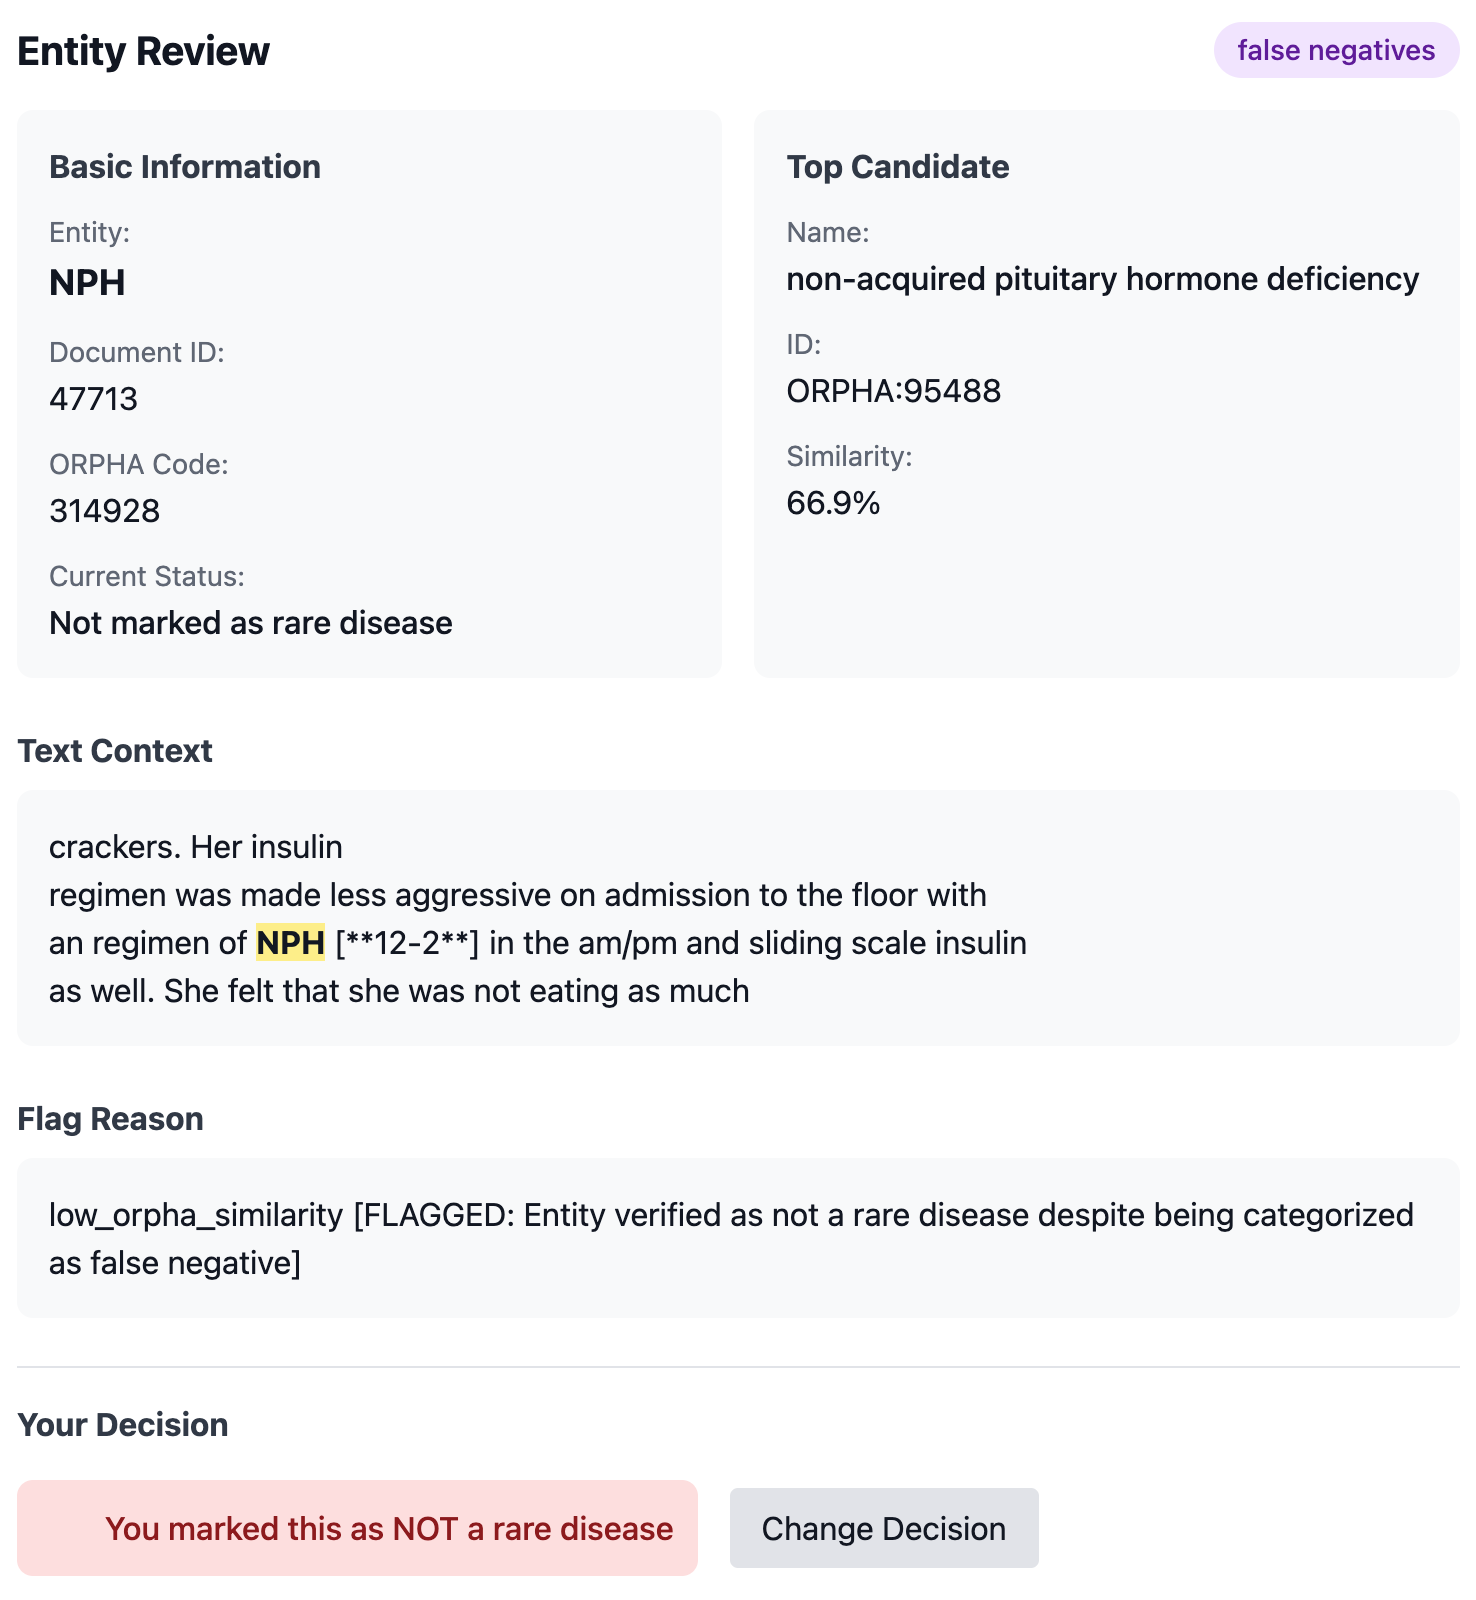
\includegraphics[width=1.0\textwidth]{figs/AnnotationUI.png}
    \caption{\textbf{Example of Inappropriate Annotation in Noisy Dataset.} We note that while NPH as an abbreivation can be related to "normal pressure hydrocephalus" or other related conditions in the Orphanet ontology as annotated by \cite{dong2023ontology_poor_annotations}, NPH here in this context is actually referring to neutral protamine hagedorn, a type of insulin used to treat diabetes. }
    \label{fig:ex_annotation}
\end{figure}

% Run a blind experiment? MedStudent for comparison and review?
\begin{table}[h!]
\centering
\begin{tabular}{l c c c}
\hline
\textbf{Metric} & \textbf{Initial} & \textbf{Human Corrected} & \textbf{RDMA \& Human} \\
\hline
Total Documents & 117 & 117 & 117 \\
\textbf{Total Number of Annotations Re-reviewed} & N/A & \textbf{333} & \textbf{122} \\
\textbf{Total Unique Rare Diseases} & 192 & \textbf{120} & \textbf{135} \\
Documents with Annotations & 117 & 117 & 117 \\
Avg. Unique Rare Diseases per Note & 1.64 & 1.03 & 1.15 \\
Avg. Word Count Per Note & 1,897 & 1,897 & 1,897 \\
\hline
\end{tabular}
\caption{Dataset Comparison: Initial Processed Dataset vs. Human Corrected vs. RDMA \& Human approaches. Human correction reduces the number of unique rare diseases from 192 to 120 (-37.5\%), likely removing false positives. The RDMA \& Human approach recovers some annotations to 135 (+12.5\% from human-only), suggesting it captures valid rare diseases missed in the initial set of annotations. \textbf{Ultimately, RDMA reduces the total number of annotations requiring re-review by a human by over 63\%.} }
\label{tab:human_v_rdma&human_stats}
\end{table}


\begin{table}[htbp]
\centering
\begin{tabular}{lcc}
\toprule
\textbf{Metric} & \textbf{RDMA Only} & \textbf{RDMA \& Human} \\
\midrule
Cohen's Kappa & 0.46 & 0.81 \\
F1 Score & 0.74 & 0.94 \\
Precision & 0.92 & 0.92 \\
Recall & 0.62 & 0.96 \\
Accuracy & 0.72 & 0.93 \\
\bottomrule
\end{tabular}
\caption{RDMA Dataset Refinement Step Agreement with Human Reviewers. While the initial RDMA-only approach shows highly imperfect performance, our RDMA with human supervision setup achieves substantially higher accuracy and agreement across all metrics. Cohen's Kappa improves from 0.46 (moderate agreement) to 0.81 (almost perfect agreement), while F1 score increases from 0.74 to 0.94, and accuracy jumps from 0.72 to 0.93. These metrics should be interpreted with nuance, as our approach prioritizes efficiency by having RDMA first identify annotations highly likely to be incorrect for human review, avoiding the time-intensive task of re-examining every annotation as shown in Table \ref{tab:human_v_rdma&human_stats}.}
\label{tab:rdma_agreement}
\end{table}


\begin{figure}[h]
    \centering
    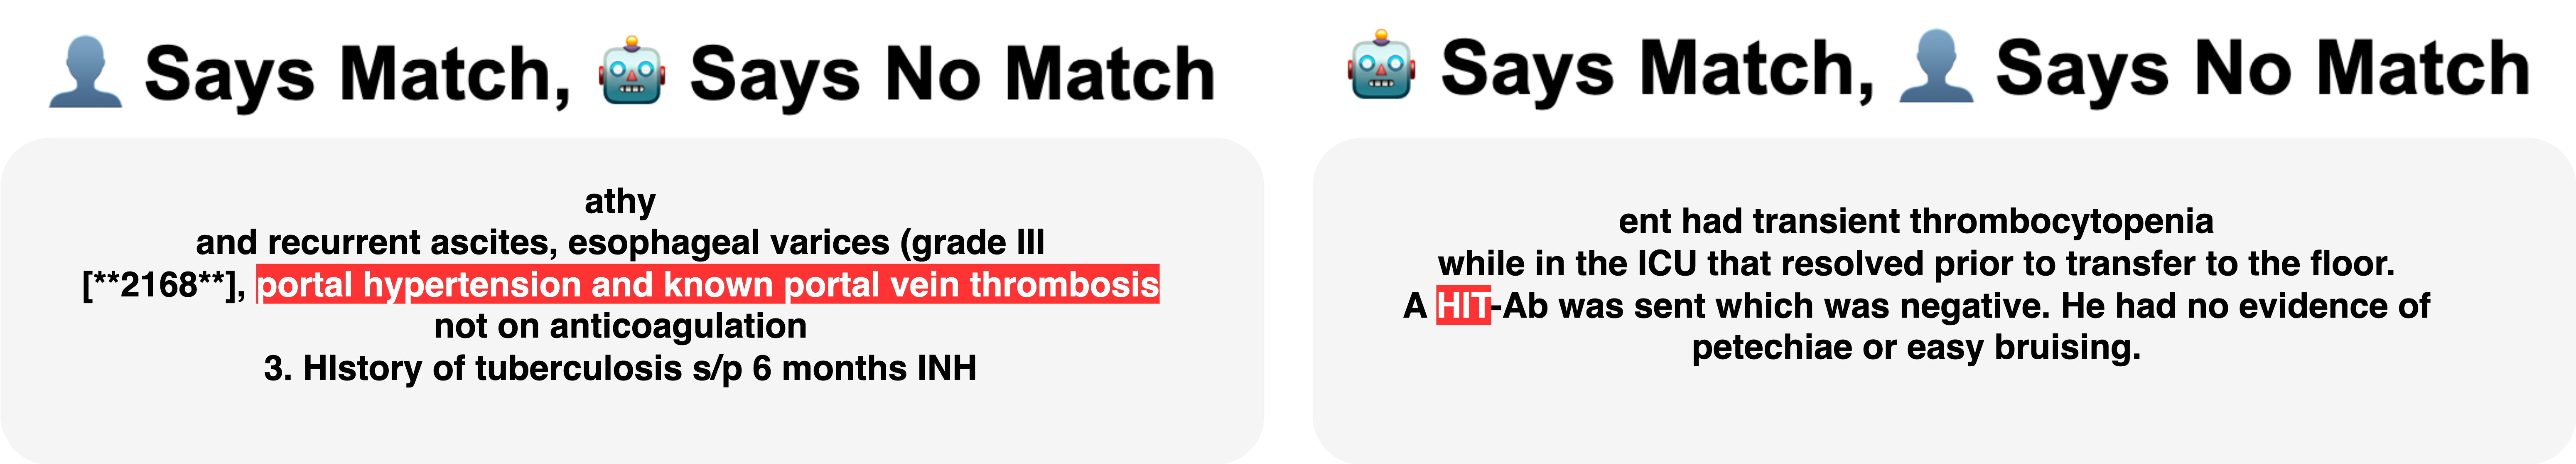
\includegraphics[width=1.0\textwidth]{figs/DisagreementSupervisorVHuman.drawio.png}
    \caption{\textbf{Failure Modes of RDMA in Rare Disease Mining.} When reviewing existing annotations, we showcase two cases where our human annotator disagrees with RDMA's refinement step. Specifically, we see that our refinement agent fails to classify portal vein thrombosis as a rare disease, primarily because its Orphanet listing "Non-cirrhotic and non-tumoral portal vein thrombosis" does not exactly match the entity "portal vein thrombosis". On the other hand, while the agent is able to classify "HIT" as "heparin induced thrombocytopenia", it does not capture the context "which was negative" properly.}
    \label{fig:annotator_agreement_qualitative}
\end{figure}


% min 500 better than no_min now for recall reasons
% Exact Match Metrics (Numeric ORPHA ID):
%   Precision: 0.5513
%   Recall: 0.3007
%   F1 Score: 0.3891
%   TP/FP/FN: 43/35/100

% Fuzzy Match Metrics (Disease Entity Names):
%   Precision: 0.5513
%   Recall: 0.2337
%   F1 Score: 0.3282
%   TP/FP/FN: 43/35/141
%   Entity matches found: 43


% \textbf{Table 2:} RDMA efficiently corrects dataset annotation errors. Our clinician found multiple mislabeled terms in clinical notes from \citep{dong2023ontology_poor_annotations}, such as "MR" incorrectly tagged as "Multicentric reticulohistiocytosis." While we filtered these errors in our initial evaluation, we also discovered many unannotated rare diseases. Under human guidance, the supervisor agent leverages Orphanet to identify genuine rare disease mentions among potential false positives to produce more accurate performance metrics.


